\begin{center}
% Correzione 2: Ridimensiona il diagramma per adattarlo alla larghezza della pagina
\resizebox{\textwidth}{!}{%
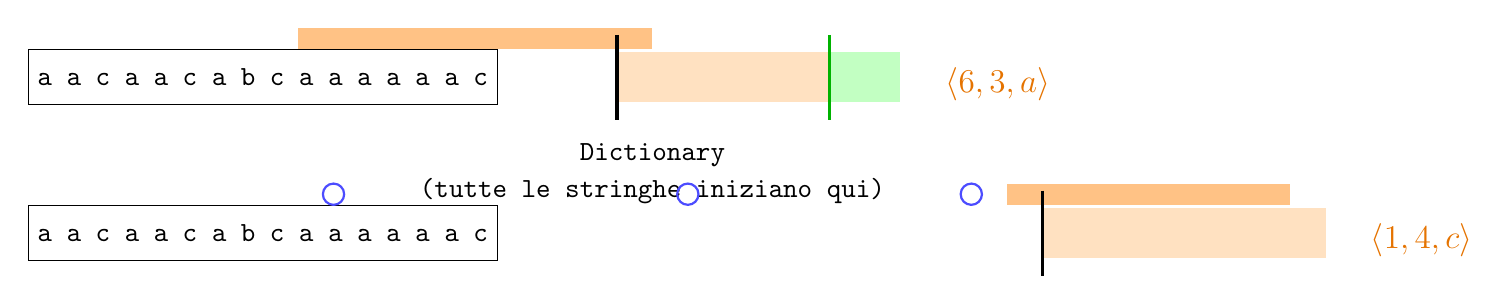
\begin{tikzpicture}[every node/.style={font=\ttfamily}, scale=0.9]

% Correzione 1: Rinominato \text in \diagramtext per evitare conflitti
\def\diagramtext{a a c a a c a b c a a a a a a c}
\def\startx{0}
\def\ytext{0}
\def\ystack{-2.2}

% Mostra la prima riga (testo completo)
% Correzione 1: Usa la macro \diagramtext
\foreach [count=\i] \char in \diagramtext {
    \node[draw, minimum size=0.7cm] at (\startx + \i, \ytext) {\char};
}

% Finestra di ricerca
\fill[orange!80, opacity=0.6] (\startx + 1.5, \ytext + 0.4) rectangle ++(5,0.3);

% Match trovato nella finestra
\fill[orange!30, opacity=0.8] (\startx + 6, \ytext - 0.35) rectangle ++(3,0.7);

% Match corrente nel lookahead buffer
\fill[green!40, opacity=0.6] (\startx + 9, \ytext - 0.35) rectangle ++(1,0.7);

% Linea divisoria tra finestra e buffer
\draw[very thick] (\startx + 6, \ytext + 0.6) -- ++(0,-1.2);

% Linea verde alla fine del match
\draw[very thick, green!70!black] (\startx + 9, \ytext + 0.6) -- ++(0,-1.2);

% Output tripla
\node[anchor=west, text=orange!90!black, font=\large\bfseries] at (\startx + 10.5, \ytext - 0.1) {$\langle 6,3,a\rangle$};

% Etichetta "Dictionary"
\node at (\startx + 6.5, \ytext - 1.1) {\bfseries Dictionary};
\node at (\startx + 6.5, \ytext - 1.6) {(tutte le stringhe iniziano qui)};

% Riga sottostante
% Correzione 1: Usa la macro \diagramtext
\foreach [count=\i] \char in \diagramtext {
    \node[draw, minimum size=0.7cm] at (\startx + \i, \ystack) {\char};
}

% Cerchi blu
\foreach \i in {2, 7, 11} {
    \draw[blue!70, thick] (\startx + \i, \ystack + 0.55) circle (0.15);
}

% Secondo match in basso
\fill[orange!80, opacity=0.6] (\startx + 11.5, \ystack + 0.4) rectangle ++(4,0.3);
\fill[orange!30, opacity=0.8] (\startx + 12, \ystack - 0.35) rectangle ++(4,0.7);

% Linea di separazione
\draw[very thick] (\startx + 12, \ystack + 0.6) -- ++(0,-1.2);

% Output secondario
\node[anchor=west, text=orange!90!black, font=\large\bfseries] at (\startx + 16.5, \ystack - 0.1) {$\langle 1,4,c\rangle$};

\end{tikzpicture}
} % Chiusura del \resizebox
\end{center}